\chapter{尾砂胶结充填体力学特性研究}
示例内容

\section{尾砂胶结充填体的物理力学性能及胶凝机理}
本文拟通过室内实验,建立中关铁矿全尾砂胶结充填体的损伤本构方程和损伤演化方程,利用充填体与围岩的能量匹配分析得到满足中关铁矿实际开采条件的最佳强度和配比,从而降低矿山生产成本。

在室内实验研究的基础上,对中关铁矿首先开采的-230中段进行数值模拟,对其采场结构参数进行优化,得到阶段空场嗣后充填采矿法的最佳采场结构参数,为矿山的设计、生产提供依据。


\subsection{尾砂胶结充填体的物理力学性能}
示例内容

\subsection{尾砂胶结充填体的胶凝机理}
	\begin{figure}[!htbp]
	\centering
	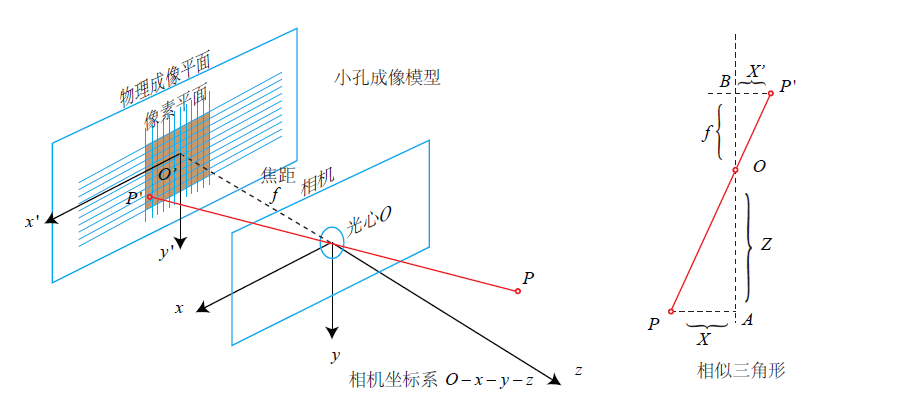
\includegraphics[width=0.80\textwidth]{myfigures/slam-01.png} %1.png是图片文件的相对路径
	\caption{针孔相机模型} %caption是图片的标题
	\label{slam-01} %此处的label相当于一个图片的专属标志,目的是方便上下文的引用
\end{figure}
